\section{Revisión de Literatura}
\subsection{Cadena de búsqueda}
\lipsum[1-4]
\subsection{Criterios de inclusión y Exclusión}
\lipsum[1-4]
\subsection{Extracción de Información}
\subsubsection{Criterios de Calidad}
\lipsum[1-4]
\subsubsection{Amenazas de Validez}
\lipsum[1-4]
\subsection{Discusión}
\citeauthor{dawkins_biology_2016} (\citeyear{dawkins_biology_2016}) afirma que agnosticismo es una filosofía incompleto. \citeauthor{nogueira2017image} (\citeyear{nogueira2017image}) contradice la anterior afirmación y presenta un ejemplo. Finalmente, se ha demostrado que es un filosofía válida \parencite[ver pag 92]{priandana2018backprop}. "El agnosticismo indica que hay un 50\% de verdad en la tesis uno y en la tesis dos" \textcite{nogueira2017image}. La Figura \ref{fig:arquitecturaRedConv} representa una red neuronal convolucional tradicional. \textcite{saha2018} afirma lo siguiente.

\begin{figure}[h!]
    \centering
    % scale, width=\columnwidth
    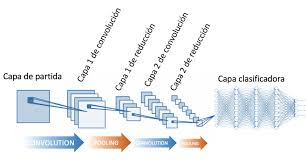
\includegraphics[width=0.7\textwidth]{imagenes/convnet.jpeg}
    \caption{Arquitectura Red Neuronal Convolucional}
    \footnotesize{Imagen tomada de \textcite[Capítulo 1, pág. 23]{nogueira2017image}}
    \label{fig:arquitecturaRedConv}
\end{figure}

\lipsum[3] La Figura \ref{fig:autoencoder_Estructura} muestra algo intersante \parencite{alberti2018} 23.5\% esto no aparecera en el pddf.

% Insertar figura 
\begin{figure}[h!]
    \centering
    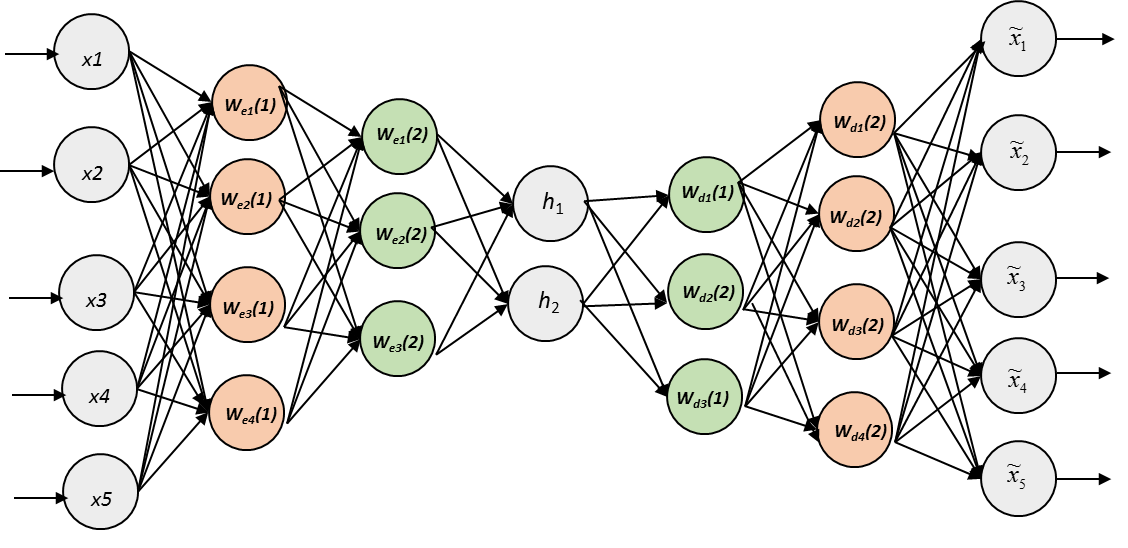
\includegraphics[width=\textwidth]{imagenes/autoencoder.png}
    \caption{Estructura de un Autoencoder}
    \label{fig:autoencoder_Estructura}
\end{figure}
